\documentclass[letterpaper,10pt]{article}
%\usepackage{hyphenat}

\usepackage[margin=1.1in]{geometry}


% For angular brackets
\usepackage{textcomp}
% Skip the indents for every paragraph
\usepackage{parskip}
\usepackage{epsfig,endnotes}
\usepackage[T1]{fontenc}
\usepackage{times}
\usepackage[square,comma,numbers,sort&compress]{natbib}
\usepackage[breaklinks,colorlinks]{hyperref}
\hypersetup{citecolor=blue,linkcolor=blue}
\usepackage{listings}
%\usepackage[outputdir=latex.out]{minted}
\usepackage{endnotes,graphicx,fancyvrb,multirow}
\usepackage{booktabs}
\usepackage{underscore}
\usepackage{amssymb}
\usepackage{tikz}
\usetikzlibrary{shapes,arrows,shadows,matrix,positioning,fit}


\newcommand\todo[1]{\textcolor{red}{TODO: #1}}
\newcommand\note[1]{\textcolor{red}{NOTE: #1}}

\newcommand\ic[1]{\texttt{#1}}
\newcommand\red[1]{\textcolor{red}{#1}}

\newcommand\para[1]{\vspace*{5pt} \noindent \textbf{#1}}
\newcommand\TODO{\textcolor{red}{TODO}}

\newenvironment{code}
{\begin{center}
	\fontfamily{pcr} \selectfont
    \begin{tabular}{|p{0.9\textwidth}|}
    \hline
	\\[-8pt]
    }
    {
	\\[-8pt]
	\\
	\hline
    \end{tabular}
    \end{center}
}


\newenvironment{temporary}{\par\color{blue}}{\par}


\newcommand{\squishenumerate}{
   \begin{enumerate}
    { \setlength{\itemsep}{0pt}      \setlength{\parsep}{3pt}
      \setlength{\topsep}{3pt}       \setlength{\partopsep}{0pt}
      \setlength{\leftmargin}{2em} \setlength{\labelwidth}{1em}
      \setlength{\labelsep}{0.5em} } }

\newcommand{\squishenumerateend}{
    \end{enumerate}  }

\newcommand{\squishlist}{
   \begin{list}{$\bullet$}
    { \setlength{\itemsep}{0pt}      \setlength{\parsep}{3pt}
      \setlength{\topsep}{3pt}       \setlength{\partopsep}{0pt}
      \setlength{\leftmargin}{2em} \setlength{\labelwidth}{1em}
      \setlength{\labelsep}{0.5em} } }

\newcommand{\squishlisttwo}{
   \begin{list}{$\bullet$}
    { \setlength{\itemsep}{0pt}    \setlength{\parsep}{0pt}
      \setlength{\topsep}{0pt}     \setlength{\partopsep}{0pt}
      \setlength{\leftmargin}{2em} \setlength{\labelwidth}{1.5em}
      \setlength{\labelsep}{0.5em} } }

\newcommand{\squishend}{
    \end{list}  }
    

\newcommand{\enablecomments}{0}

\ifnum\enablecomments=1
  \newcommand{\congyu}[1]{\textcolor{blue}{\textbf{CL: #1}}}
  \newcommand{\paul}[1]{\textcolor{purple}{\textbf{PN: #1}}}
  \newcommand{\yi}[1]{\textcolor{orange}{\textbf{YS: #1}}}
  \newcommand\pf[1]{\textcolor{red}{PF: #1}}
\else
  \newcommand{\congyu}[1]{}
  \newcommand{\paul}[1]{}
  \newcommand{\yi}[1]{}
  \newcommand\pf[1]{}
\fi
 

\usepackage{fancyvrb}


\begin{document}

\begin{center}
    {\LARGE{Project 1: Dynamic testing}}\\
  \vspace*{10pt}
  {\Large{CS408, Spring 2026}}\\
    \vspace*{10pt}

  {\large{\textbf{Group Project (140 points)\\
        \vspace*{3pt}
        Due date: February 27, 2026}}}\\
      \vspace*{15pt}
\end{center}



\if 0
\begin{temporary}

\section{TODO}
\begin{itemize}
  \item ...
\end{itemize}

\section{DONE}
\begin{itemize}
  \item ...
\end{itemize}

\end{temporary}
\fi

\section{Project overview}

In this project, you will implement a testing framework that includes a testing scheduler and bug detectors for applications.

%The testing framework will have a testing scheduler and
%a dynamic data race detector. Note that each part has its own due date.

The testing scheduler will be responsible for running the application with different schedules.
This tool is related but significantly simpler than the CHESS tool discussed in class.
Exploring different schedules will allow testers to uncover concurrency bugs that, for instance, cause the application to trigger an assertion violation or
crash under a subset of the interleavings.
% The testing scheduler will support different policies responsible for deciding which interleavings to execute on each test iteration.

In addition to the testing scheduler, you will also implement support for several bug detectors that will analyze each execution of the target program.
This component will allow the framework to detect crashes, performance bugs, memory errors, and data races.

%The dynamic data race detector will complement the testing scheduler to detect
%data races in each execution of the target program. The data race detector will
%rely on the happens-before technique.

Read the assignment entirely before starting any work on it.

This project is a group project -- collaboration is only allowed between members of the same group. Check the course academic integrity rules for additional details.
Groups have to be registered according to the instructions provided in Ed.


% \subsection{Group registration}
% \label{sec:group}
%
% Find group members to create a group of 3 students. Only exceptionally will
% groups of 2 students be allowed. Group membership cannot change during the
% semester.
%
% Once you determine your group membership, please send an email to Jonathan
% Rosenthal <rosenth0@purdue.edu> with the full name and username of each group
% member. Make sure you use your official Purdue email address when sending the
% email and ensure you CC your other group members in the email. Only one email
% should be sent per group. Your subject must include the prefix ``[CS408] Group membership''.
%
% Students that cannot find a group should send an email to Jonathan Rosenthal
% stating this so that they can paired with other students by the course staff.


\section{Project setup and development workflow}

Please follow the instructions in \autoref{sec:appx:setup} to \textbf{clone}, \textbf{setup}, and regularly \textbf{update} your Github classroom private repository.

Use this link \url{https://classroom.github.com/a/AXaiz8nQ} to accept the assignment on GitHub classroom.


\vspace*{10pt}

\fbox{
\begin{minipage}{\textwidth}
\textbf{REQUIREMENT:} Your private GitHub classroom repository is going to be used to (a) help staff provide support to students when there are questions about their project, (b) help students backup and cooperate within each group, (c) investigate cases of plagiarism, and (d) investigate cases of uneven contributions among group members.

Hence, in this course, students are \textbf{required} to use GitHub classroom and regularly commit and push their updates (e.g., approximately every 2 hours of work). Not following this requirement will lead to \textbf{partial or total loss of points} in the project's final grade.
\end{minipage}
}

\vspace*{10pt}

\textbf{PARTICIPATION EXPECTATIONS:} Every group member must participate
throughout the project duration equally and be familiar with all
components of the work delivered by the group.

\para{Responsibility.}
For each function you implement or modify, please write your Purdue alias as a comment above the function.
If your code does not contain any functions (for example, if it's just Python code), you should include your alias as a comment at the end of the file.
There is no need to include your alias other than functions and statements, such as global variable declarations.

\subsection{Starting}

Use the package provided in the starting git repository to implement the
project. This project has to be done in the C and Python languages, and your solution must be
able to run in \texttt{data.cs.purdue.edu}.

% \para{Git repository.} It is recommended the use of a git repository. However,
% you should ensure that permissions are set correctly such that only group
% members can access the git repository.

\subsection{Workflow}

To facilitate the implementation process, we present a concise guide outlining the essential components required. A testing framework must be constructed to facilitate the automatic testing of the target programs.
Refer to \autoref{fig:workflow} for a visual representation of the workflow. To ensure the seamless operation of the framework, three main parts need to be prepared.
%, and the framework implementation needs to be completed.
The framework is expected to run the test scheduler and selected bug detectors on the target programs automatically.

The test scheduler, as depicted in \autoref{fig:testscheulder}, comprises three distinct parts that you will need to implement.
The first part, "Interposing pthread calls," requires familiarity with the \ldp instrumentation method (i.e., a way to control the tested application).
%The third part mandates the implementation of two algorithms to enable the proper execution of the test scheduler. Please read the section ~\autoref{sec:schedule} carefully for more information.
The third part mandates the implementation of one algorithm (Random) to enable the proper execution of the test scheduler.
Please read the \autoref{sec:schedule} carefully for more information.

\begin{figure}[!htb]
   \begin{minipage}{0.48\textwidth}
     \centering
     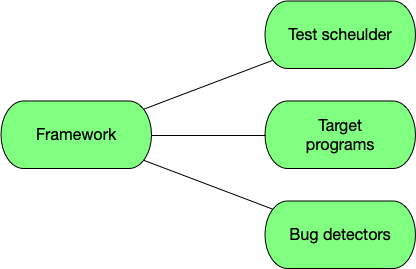
\includegraphics[width=.7\linewidth]{figures/work_flow.png}
     \caption{Main Parts}\label{fig:workflow}
   \end{minipage}\hfill
   \begin{minipage}{0.48\textwidth}
     \centering
     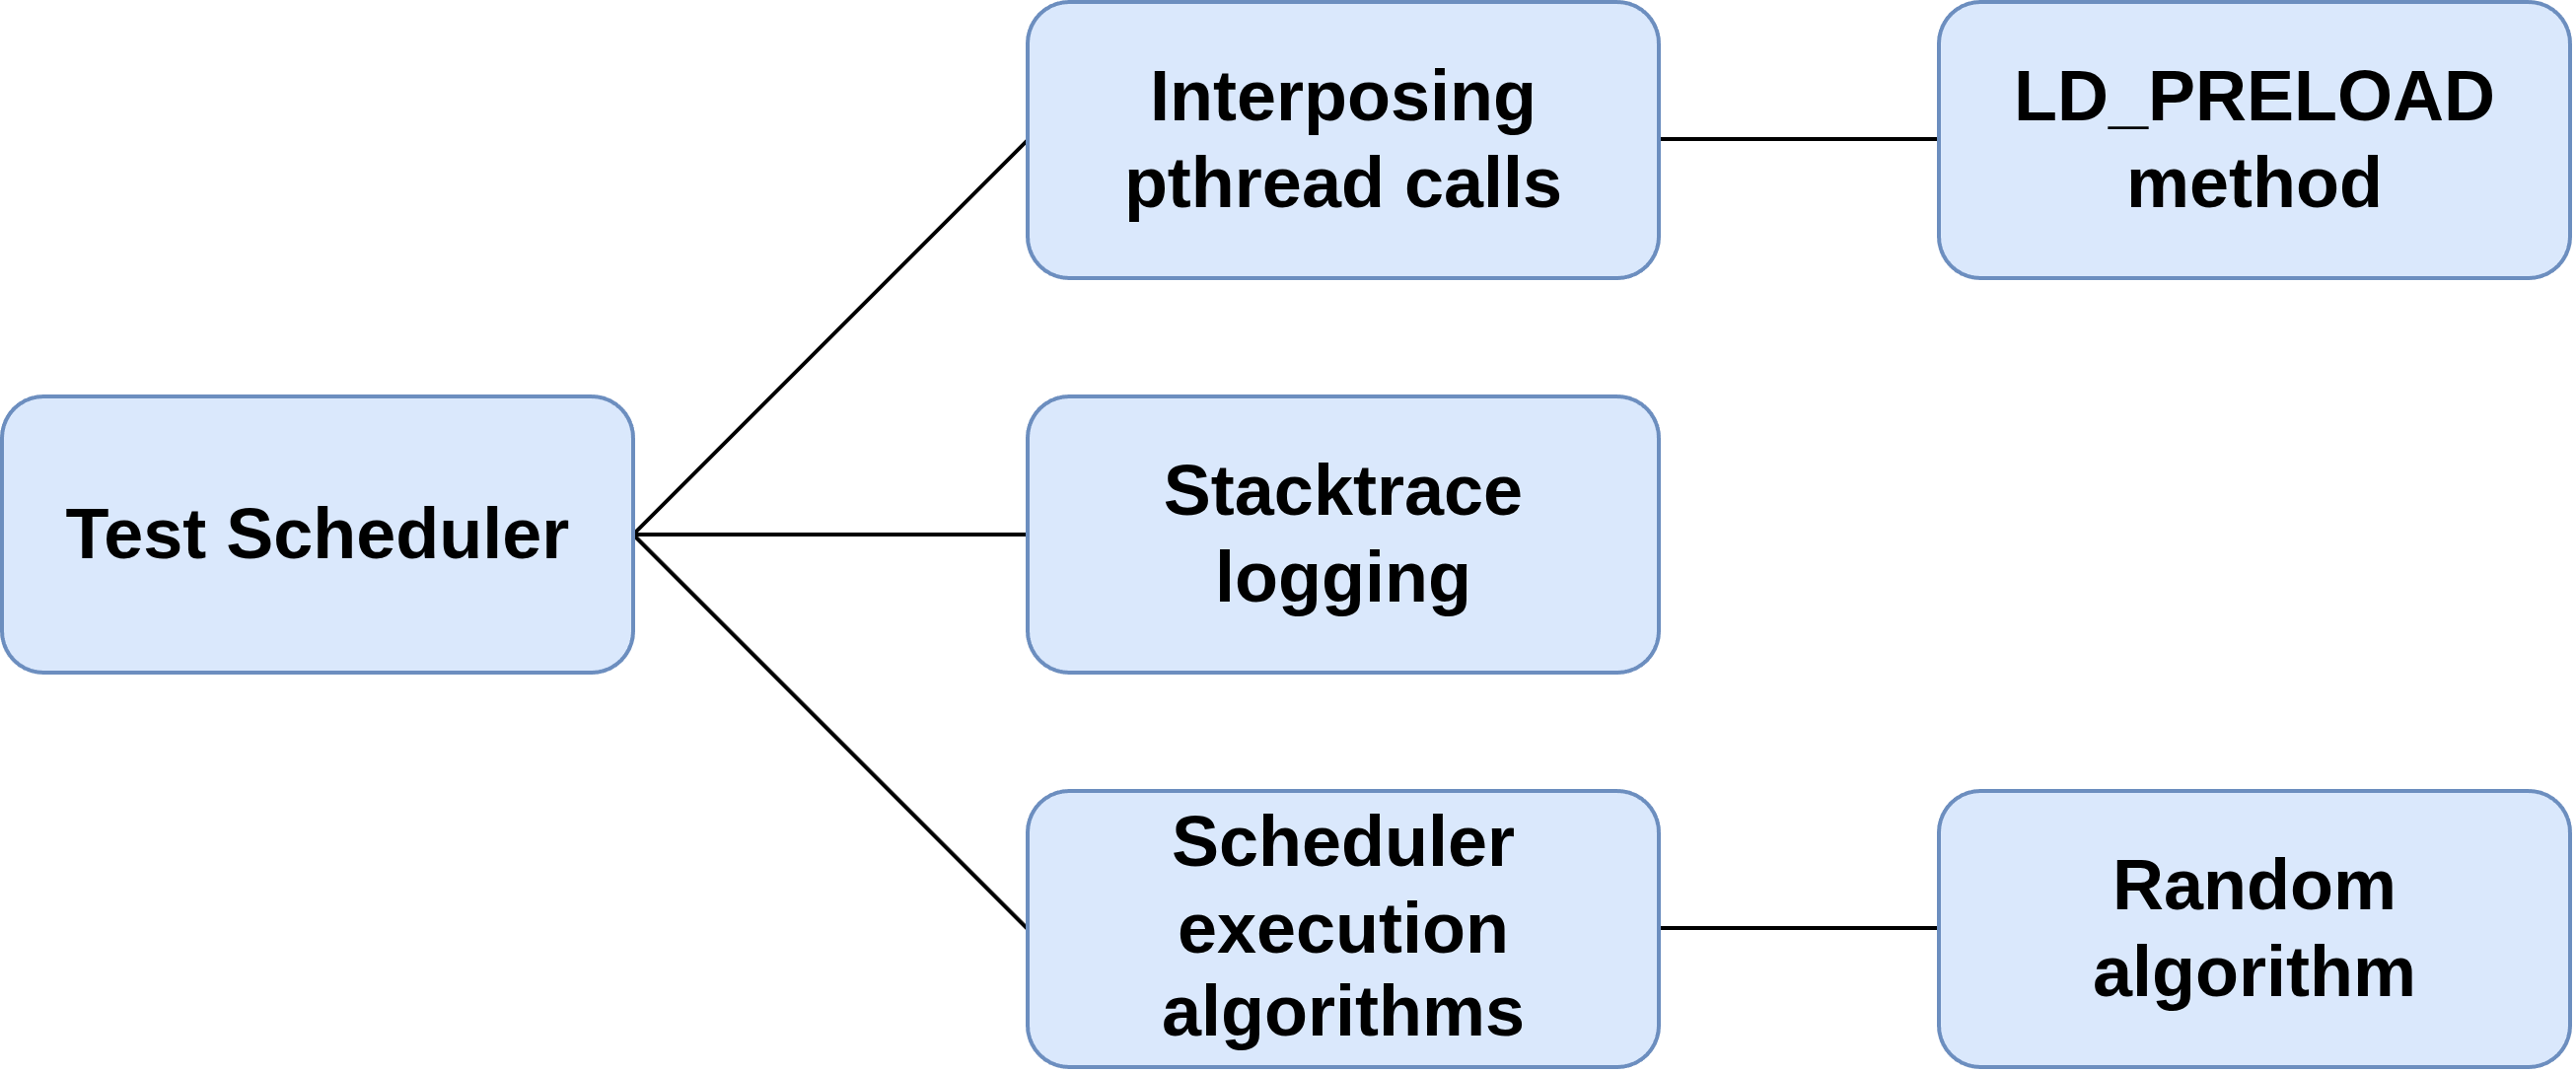
\includegraphics[width=.7\linewidth]{figures/scheduler_work_flow.png}
     \caption{Test Scheduler}\label{fig:testscheulder}
   \end{minipage}
\end{figure}

\subsection{Framework interface}
\label{sec:interface}

The dynamic testing framework that you build needs to satisfy the following interface for grading purposes:

%\todo{The binary for "./dctest" does not exist in the skeleton. What is it referring to?}
\begin{Verbatim}[fontsize=\small]
  $ python3 framework.py -s <none|random> -n <iterations> -st <true|false>
            -seed <seed>
            <target> [<target args>]
\end{Verbatim}

%\begin{Verbatim}[fontsize=\small]
%  $./dctest -s <none|pct|random> -n <max_iterations> -st <true|false>
%            -seed <seed> -dd <true|false>
%            <target> [<target args>]
%\end{Verbatim}


The arguments have the following meaning:

\begin{itemize}
  \item
  -s <none | random>: determines the testing schedule policy, which can be no
   schedule instrumentation (``none'') or random (``random'').
  \item
  -n <iterations>: defines the number of iterations of the target program
   that the framework will execute. Must be an integer greater than zero.
  \item
  -st <true | false>: defines whether stacktrace logging is enabled or not.
  \item
  -seed <seed>: defines the integer seed for the testing scheduler.
  %\item
  %-dd <true | false>: specifies whether the data race detector is enabled or not.
  \item
  <target>: target program that the framework will test.
  \item
  <target args>: optional command-line arguments for the \textit{target program}.
\end{itemize}

The skeleton framework provided already includes the code necessary to
receive and process these arguments.

The testing framework will run the target program several times (as specified by ``iterations''). 
For each iteration, the testing framework prints the
output of the program to standard output.\\

\autoref{sec:schedule} explains the output of
the testing framework in more detail.

The framework shall return the following exit codes:
\begin{itemize}
  \item 0: Success case. Framework executed at least one iteration of the program, and
  the program returned exit code zero for all iterations executed.
  % and, when the data race detector is enabled, no data race was found.
  \item 1: Framework received invalid arguments.
  \item 2: Program terminated with a non-zero exit value for at least one iteration.
  % or a data race was found in at least one iteration.{}
\end{itemize}


\subsection{Useful Libraries and Algorithms in ~\autoref{sec:appx:libs}}

To enhance the readability of this project, we have included several usage examples and hints for libraries and algorithms in ~\autoref{sec:appx:libs}. Note that these sections are of utmost importance and should be read thoroughly before beginning the implementation process. Doing so can significantly reduce the time and effort required to complete the project.

For successful implementation of this project, you need to understand well how programs handle threads and perform thread synchronization. 
%it is imperative to possess a comprehensive understanding of how programs handle threads and perform thread synchronization. 
Refer to \autoref{subsec:appx:pthreads} for crucial API usage and hints for the \pthread library to execute synchronization operations and thread management.

In order to implement the testing scheduler, the \ldp methods must be utilized to intercept the \pthread calls made by the target program. A simple example of the \ldp method is provided in the appendix section to facilitate the implementation process in \autoref{sec:interposing}.

% Removed: 09/09/2025 due to simplfy the question
%The PCT algorithm is a uniprocessor scheduler that must be implemented in ~\autoref{sec:schedule}.
%To successfully complete this section, it is recommended to follow the workflow and requirements outlined in \autoref{subsec:appx:pct}.

\section{Testing scheduler (100 pts)}
% (120 pts)}
\label{sec:schedule}


To build the testing scheduler, you will need to implement a library that will
intercept the \pthread calls made by the target program using the \ldp
method (\autoref{subsec:appx:ldpreload}). This method will ensure that your testing
framework takes control of the program at these critical points in its
execution. 
In particular, it will allow us to add additional scheduling
constraints to the program, which will cause the execution of other interleaving.
\textbf{Noted that the testing scheduler can be implemented entirely inside this library.}

For this section, you will need to modify or implement the following files:
\begin{itemize}
%\item \texttt{testlib.h} and \texttt{testlib.c}
\item \texttt{testlib.c}
\item \texttt{coverage\_tests\_helper.py}
\item testing programs in \texttt{coverage\_tests/} directory
\end{itemize}

\autoref{sec:assumptions} lists several
assumptions that you can make about the target program. \textbf{Your testing framework
does not need to support applications that do not satisfy those assumptions.}


\subsection{Interposing \pthread calls}
\label{sec:interposing}

You will need to interpose all \pthread calls mentioned in \autoref{subsec:appx:pthreads} using the LD_PRELOAD method(\autoref{subsec:appx:ldpreload}). LD_PRELOAD will allow your
framework to have hook functions called on key points of the target
program regarding thread management and thread synchronization. The target
program should still see the correct semantic of the \pthread calls.

\textbf{NOTE:} In the grading, we will not use \textit{pthread_join} or other functions not listed in the handout in the test programs.

For example, you should define the \textit{pthread_create} call in your test
library and ensure that the original \textit{pthread_create} call is called
within your function. Your \textit{pthread_create} will be the right place for
you to add instrumenting code just before the original \textit{pthread_create}
is called and just after the original \textit{pthread_create} function returns
(to your library). You must intercept every \pthread function in appendix
\autoref{subsec:appx:pthreads}.

In the case of \textit{pthread_create}, you should also modify the
\textit{start_routine} function pointer, which is a parameter given to
\textit{pthread_create}.
Your modification needs to ensure that when a process creates a a new thread,
your framework is immediately notified and gets the opportunity to run code
before the original (program) \textit{start_routine} is actually called by \pthread.
Furthermore, this will also give the opportunity to detect when the
\textit{start_routine} returns. This is important because your scheduler
needs to know (and act) when threads are created and when they terminate.

Note that your framework will itself have concurrent code, i.e.,
code that multiple threads can concurrently execute. So you need to ensure that you
synchronize your code whenever necessary, and you need to do so using the
original synchronization functions.

Your framework needs to print the following types of log entries to
stdout when the target program executes \pthread functions:
\begin{itemize}
\item ``CALL <function_name>([list_of_function_args])''
\item ``RETURN <function_name>([list_of_function_args]) [= <return_value>]]''
\end{itemize}

In addition to function-related log entries, if a thread is created or exits the
following thread-related log entries should be printed to stdout:
\begin{itemize}
\item ``THREAD CREATED [<thread \#>, <thread ID>]''
\item ``THREAD EXITED [<thread \#, <thread ID>]''
\end{itemize}

The thread ID is provided by the OS and can be determined by calling the function \textit{gettid()}. \textit{thread \#} is the sequential thread count number. The main thread is thread 0, and for every new thread created by the program, the value should be incremented by one. You must keep track of the thread sequential number with a global counter.


As an example, your testing framework should print the following log entries, possibly in a
different order and with different argument values, when \textit{pthread_create}
is invoked by the target program:

\begin{verbatim}
  CALL pthread_create(0x100010, 0x1000030, 0x1000, 0x1000)
  RETURN pthread_create(0x100010, 0x1000030, 0x1000, 0x1000) = 0x0
  THREAD CREATED (2, 103)
  THREAD EXITED (2, 103)
\end{verbatim}

\textit{pthread_create} can generate up to 4 log entries because a new thread is
eventually created and eventually exits, i.e.,
if the \textit{starting_function} returns or if \textit{pthread_exit} is called. The
other \pthread functions can only generate at most 2 log entries.

\textbf{NOTE:} You do not need to print ``THREAD EXITED'' messages when the process exits, only
when individual threads terminate by either returning from the starting function
or calling \textit{pthread_exit}.

% \if 0
% Unlike the other \pthread calls, \textit{pthread_create} receives a variable
% number of arguments, i.e., it is a variadic function. This requires a bit of
% extra effort in the implementation of your \textit{pthread_create} interposing
% function. In particular, to receive an arbitrary number of arguments and invoke
% the original \textit{pthread_create}  with an arbitrary you should use the
% variadic functions defined in ``stdarg.h''. You can find an example of how this
% can be achieved in \textit{man va_start}.
% \fi

The log entry print operations need to be performed immediately before calling
the original function and immediately after it returns. Log entries should
print function arguments in hexadecimal, and thread sequential numbers and IDs should be printed in decimal, using the
exact format shown in the example above. This is important for grading purposes.

If the program also prints output to stdout the output of your testing tool and
the program might be intertwined. However, you need to make sure your output is
protected internally with locks, i.e., your library only makes one
\textit{printf} to the console at a time (even if the application concurrently
invokes several \pthread functions). Furthermore, you should flush the stdout
stream with \textit{fflush(stdout)} after each \textit{printf}.


\subsection{Stacktrace logging on \pthread invocations}

In addition to printing the log entries for each \pthread event described in section
\autoref{sec:interposing}, you will need to print the stacktrace of the target
program. This form of logging must be togglable with the
framework argument ``-st''.
%the variable \TODO in \textit{common.h}.
You must print the stacktrace using the provided library \textit{libunwind}.

The following program demonstrates the use of the \textit{libunwind} library
to print a stacktrace of a C program:

\VerbatimInput{unwind-test2.c}

You can compile the above program by adding a main and an invocation to stacktrace() with the following command:

\begin{verbatim}
  $ gcc -l unwind -o unwind-tests unwind-test.c
\end{verbatim}

Or, you can use the unwind library in the skeleton:

\begin{verbatim}
  $ gcc -o test ./unwind-test.c ./libunwind/lib/libunwind.a -I./libunwind/include
\end{verbatim}

You should print the stacktrace of the target program at every point where it
invokes a \pthread call. For every \pthread function invocation, you must print
only once the stacktrace and it must be immediately after the respective CALL
log entry. Do not print a stacktrace when \textit{starting_function} enters or
exits.

The stacktrace you print must only include the code of the target program. In
particular, it must not include any code of the testing framework.


\subsection{Algorithm: Random}

Some testing algorithms force certain schedules to execute, but such algorithms tend to be more complex to implement. 
For this project you will instead implement a random scheduler algorithm, which will disturb the execution of threads by calling the sleep
function with pseudo-random durations. For your project, you will need to
implement the random scheduler by calling the following usleep function at every
scheduling point:

\begin{verbatim}
  usleep((rand()%1000) * 1000);
\end{verbatim}


The random testing scheduler must make the above sleep call when and only when:
\begin{itemize}
  \item A \pthread call listed in \autoref{subsec:appx:pthreads} is invoked or returns
  \item A thread starts executing
  \item A thread terminates
\end{itemize}

The skeleton code already does the initialization of the random number generator
based on the framework \textit{-seed} argument. Do not initialize
the random generator with your own calls to the function \textit{srand} or
similar. This would interfere with grading.

%% Removed, 2025/09/03 due to simplfy the work and focus on testing
%\subsection{Algorithm: PCT}
%
%The PCT algorithm is a uni-processor scheduler.
%This means that it
%only allows one thread of the program to run at any time, unlike the random testing algorithm.
%The challenging task for the scheduler is to ensure that one and only one thread is
%able to make progress at any point in time.
%
%It is also a priority-based scheduler, which means that each thread will be
%assigned a priority, and the scheduler always runs the highest priority
%thread in a \textbf{runnable state}.
%
%The PCT algorithm is deterministic, i.e., for the same testing seed it should always execute the same exact interleaving of threads. Your implementation must not call any random sleep function for this algorithm.
%
%For this project, similarly to the random testing scheduler,
%the PCT testing scheduler makes scheduling decisions when and only when:
%\begin{itemize}
%  \item A \pthread call listed in \autoref{subsec:appx:pthreads} is invoked or returns
%  \item A thread starts executing
%  \item A thread terminates
%\end{itemize}
%
%You can figure out the work flow of PCT by reading the simple demo in ~\autoref{subsec:appx:pct}. Please read carefully about this appendix and follow the \textbf{requirements} in it to finish your implementation. This will help you save a lot of time.

\subsection{Framework code coverage tests}
\label{sec:framework:tests}

You should create several sample multi-threaded target programs. Ensure that at
least 5 of those sample programs are buggy and 5 are non-buggy programs. Use
these programs to test your own testing framework.

Place all the testing programs in the \textit{coverage\_tests/} subdirectory and make sure
your framework has a \textit{Makefile} target called ``run\_coverage\_tests'' that will compile and run
all the test cases in your framework.

Your set of test cases must have 100\% code coverage of your testing library
for all feasible parts of the code. Include this part in your report in pdf format named \textit{report.pdf},
where you discuss the coverage over the testing library (not the entire testing
framework) you achieved. Write this report regardless of whether you achieve 100\% coverage or a lower value. If you did not manage to get 100\% coverage of the testing library, for each
region that is not covered by your test cases, explain in detail why it is not
covered. Include in your submission the test case coverage raw file produced
using gcc.

\section{Bug detectors (40 pts)}

As part of this project, you will also need to add to your testing framework
4 bug detectors: (a) a crash
detector, (b) a performance bug detector, (c) a data race detector, and
(d) a memory error detector. Most of these functions need to be implemented
outside of the testing \textit{library}.

For this section, you will need to modify or implement the following files:
\begin{itemize}
\item \texttt{framework.py}
% \item \texttt{testlib.c}
%\item \texttt{Makefile}
\item buggy programs in \texttt{detector\_tests/} directory
\end{itemize}



\subsection{Expand the framework interface}


To support these bug detectors, add a new and optional (from the user's point
of view) command line flag to the
testing framework ``-detector'' and ensure that this flag can receive a
comma-separated list of options that activate a combination of the available
detectors (``crash'', ``perf'', ``dr'', ``memory''). Any combination of the
options is valid, and they can be provided in any order. However, if ``-detector'' is
passed, there must be at least one detector in the list for the command-line options to be valid.


So a valid example would be, for instance:
\begin{Verbatim}[fontsize=\small]
  $ python3 framework.py -s random -n 5 -st false -seed 1
                         -detector crash,dr,perf ./mytarget args
\end{Verbatim}


When the detector option is passed, the framework should ignore the exit code of
the target program and instead use the result of the active detectors to
determine whether the execution was successful or not. An iteration is considered
successful if and only if none of the active detectors flags an error. If an error is detected on an iteration, the framework exits without executing the following iterations.

\textbf{NOTE:} If you meet some bugs in the iteration, please print all bugs fro the current iteration and terminate.

If the last execution triggers multiple detectors,
the framework does not need to print messages of more than one detector.


If the command-line options are not valid, the framework should
return the appropriate framework error exit value without running the test program
(\autoref{sec:interface}).



\subsection{Crash detector}

The crash detector detects illegal memory accesses, such as null pointer dereferences. These are situations that the operating system detects that make it terminate the target program.

Your framework should detect whether the target program crashed by analyzing the signal
number that caused it to terminate. This can be achieved using the ``WTERMSIG()''
macro or equivalent [9]. In practice, this detector only needs to detect the SIGSEGV signal (``'Invalid memory reference'') [10].

Make sure that you can get the signal value even when other detectors are active. In particular, make sure the crash detector is compatible with valgrind used by the memory error detector (\autoref{sec:memorydata}).
%\todo{JK, Please check that this is possible.}

On failure detected, this detector should print the message: ``DETECTOR: Crash detected.$\backslash$n''.

\subsection{Performance bug detector}

The performance bug detector will detect executions where the program execution time deviates significantly from the normal execution time. This allows the framework to detect bugs that cause the program to slow down or hang on a small \textit{subset} of interleavings.

Your detector will rely on a timeout heuristic to detect performance bugs. In a given run of the framework, the heuristic will use the average execution time of all prior iterations (of the given framework run), and consider the current execution to be a failure if it takes more than $AVG + 3$ seconds, where $AVG$ represents the average time of prior iterations. Use floating-point numbers to determine the average execution time and implement a timeout granularity of 1 ms (or smaller).

Your framework should \textit{terminate} the execution of the target program as soon as the timeout period is reached. This will ensure that the framework terminates even if the target program hangs.

Because this heuristic uses the execution time of previous iterations, this detector will always consider the first 10 interactions to be successful. In other words, it only applies the heuristic to the 11th and the subsequent iterations.

After each iteration, including the first one, your detector should print the message ``DETECTOR: Last execution time: x.yyy seconds. Average execution time: x.yyy seconds.$\backslash$n'', containing the execution time of the last execution and the average execution time of all executions (including the one that just terminated).

On failure detected, this detector should print the message: ``DETECTOR: Performance bug detected. Timeout: x.yyy seconds.$\backslash$n''.

\subsection{Memory error and data race detectors}
\label{sec:memorydata}

To simplify, you will not implement the core
components of the data race detector or memory error detector; instead, you will use
\textit{valgrind} for this purpose. In particular, use the ``memcheck'' and the ``helgrind'' options of valgrind to detect memory errors (e.g., memory leaks) and data races, respectively.

When these detectors are active, your framework should simply launch valgrind with the appropriate parameters and detect the outcome of valgrind. For the memcheck tool, use the following valgrind arguments: ``$--$tool=memcheck $--$error-exitcode=1 $--$leak-check=full'' (in addition to the target program path/arguments and other arguments that you find necessary). For the helgrind tool, use the following valgrind arguments: ``$--$tool=helgrind $--$error-exitcode=1'' (in addition to the target program path/arguments and other arguments that you find necessary).


To detect the errors, your framework will need to parse the output of these tools (either the exit value or the console output).
On error detected, the memory detector should print the message: ``DETECTOR: Memory error detected.$\backslash$n'' and the data race detector should print the message  ``DETECTOR: Data race detected.$\backslash$n''. In addition, the output of valgrind should always be printed to the console when these detectors are active.

This project must be completed using only the tools and software provided within the lab environment. The use of any external tools, including but not limited to personal software, online resources, or physical devices, is strictly prohibited unless otherwise specified by the instructor.


%\todo{JK, please check that LD_PRELOAD and valgrind are compatible. Also, please check if special parameters are necessary for them to work together.}

\subsection{Bug examples}


For each bug detector, provide a buggy program (written in C) that has a single concurrency bug
and activates a single bug detector. Write the bug examples such that they
are unlikely to trigger the concurrency bug without the testing scheduler, but
likely to trigger the bug with the testing scheduler. You can use sleeps to
control the interleavings.

In addition to controlling the interleavings, you will likely need to include a code fragment
that causes certain thread interleavings to trigger new program control paths
(of one or both threads) that execute the buggy code. This code fragment should not
include data races, except for the data race detector case. Otherwise, more than
one bug detector would detect an error/failure.

The test programs in \autoref{sec:framework:tests} have the goal of testing
the framework. In contrast, the test programs of this section have the goal of
demonstrating the use cases for the testing framework. Hence, these tests do not
need to cover well the testing framework. The test programs of both sections can
be similar or even the same if it helps, but make sure you use distinct files
for each project component.

Place all the program bug examples in the \textit{detector\_tests/} subdirectory.
In addition, make sure your framework has a \textit{Makefile} target called ``run\_detectors'' that will compile and run all the test cases in your framework.
By default, the Makefile target should run these programs using the options: ``-s random -n 100 -st false -seed 1''.
Name the test programs as follows:

\begin{verbatim}
detector_tests/crash.c
detector_tests/perf.c
detector_tests/dr.c
detector_tests/memory.c
\end{verbatim}

The programs included should be simple (e.g., less than 20-30 statements) and
easy to understand.

Also discuss this part in your report. Give the brief explanation for your programs and the test results.

% \subsection{Part 1 submission}
%
% Follow the instructions in \autoref{sec:submission} to submit part 1 by the
% part 1 due date.




% %%%%%%%%%%%%%%%%%%%%%%%%%%%%%%%%%%%%%%%%%%%%%%%%%%%%%%%%%%%%%%%%%%%%%%%%%%%%%
% \section{PART 2: Data race detector (80 pts)}
% \label{sec:datarace}
%
% Your framework will implement a happens-before data race detector that is only
% enabled when the user provides the appropriate flag to the testing framework
% (\autoref{sec:interface}).
%
% \subsection{Memory operations}
%
%
% \subsection{Happens-before data race detector}
%
%
% \subsection{Stacktrace and output format}
%
%
% \subsection{Part 2 submission}
%
% Follow the instructions in \autoref{sec:submission} to submit part 2 by the part
% 2 due date. Your part 2 submission should be fully functional and include part 1
% code, but only part 2 code will be \textit{explicitly} graded.
%
% You do not need to modify your test cases for part 2. But it is recommended for you to create new test cases that specifically test the part 2 functionality.

\section{Program assumptions}
\label{sec:assumptions}

For this assignment,
you should make the following
assumptions about the target program. These assumptions will simplify the
implementation of the testing framework:

\begin{itemize}

\item
Threads and synchronization objects are created with the default options and attributes.

\item
Every successful lock operation is eventually followed by the respective unlock operation on the same mutex.

\item
Data races do not prevent the program from progressing.

\item
The only library calls executed by the program are standard file system
operations. No system calls are made directly (e.g., \textit{syscall()} is not used).

\item The program does not use signals or signal handlers.

\item The program does not launch other programs.
In particular, the program does not
call \texttt{fork} or \texttt{execve} system calls.

\item
The program reads input from files (or does not receive any input), and all
program output is written to the standard output. Hence, you do not need to
perform any task for the program to receive input, and you do not need to worry
about clean up after each test iteration.

\item
You can assume that the program will have less than 64 threads running
at any point in time.

\end{itemize}


\section{Submission}
\label{sec:submission}

You must submit your work in a \textbf{single zip} file using
Brightspace with the following
filename format, making sure to replace \textit{username1}, \textit{username2},
and \textit{username3} with the appropriate usernames of each group member:\\
 {\hspace*{30pt}\textbf{username1_username2_username3.zip}}

Only one person in each group needs to submit the project. The most recent submission before the deadline will be graded.

Make sure you use the skeleton provided for your submission. Your submission
must include the skeleton directory provided, with the code for your framework
in the main directory. Do not rename files and use existing files whenever possible.

The submission must satisfy the following requirements:
\squishlist
 \item All your code must be written in \textbf{C and Python exclusively}. No other languages
will be allowed.
 \item Do not change code in files that explicitly say not to modify unless authorized by the course staff, use \textit{check\_modified.sh}.
 \item The framework must not rely on any external tool. The only allowed
 resources are: the standard libraries included with C, the libunwind library
 included in the skeleton, and the fragments of code in this project assignment.
 \item Include a report in pdf format named \textit{report.pdf}. You could also include some other notes for your implementation.
 \item Your submission must only include code of the group members. Do not
 consult or use any other code. Refer to the course policy on plagiarism for
 additional details about the course policy.

\squishend

The submitted package size needs to be reasonable (less than 0.5 MB uncompressed). The framework and all tests must: run in reasonable time (less than 10 min for the entire test set), use only reasonable resources, and run correctly on \textit{data.cs.purdue.edu}.

Projects delivered 5 full days ahead (February 22, 2026) of the official project due date receive 5 bonus points, as long as they score at least 50\% of the regular points.



Reminder: In accordance with the course policy, the number of late days available for the group project is the \textbf{minimum} number of late days that each group member still has available.

% For the purpose of late days, each part of this assignment is considered a
% different project. Hence, if your group still has 3 late days left at the start
% of this project and uses 1 late day for the first part, your group will only
% have 2 late days available for the second part.

\section{Grading and group member contributions}

All students are expected to \textbf{contribute equally} to the project and be \textbf{familiar
with all components of the project}. Furthermore, every group member must participate
throughout the project duration equally and be familiar with all
components of the work delivered by the group. If the staff suspects or receives
reports from group members of significantly unequal contributions to the project,
we may investigate the contribution of each student by analyzing the GitHub
classroom participation, interviewing students, and using other evidence.
Furthermore, we may decide to conduct an oral exam to all group members to
assess their knowledge on the project. The results of the exam and investigation
may lead to different grades, including grade zero, for different group members.

Please report any problems with your group as \textit{early} as possible (i.e.,
ideally well before the due date) so that we can more easily address the problem.
Reports will only be considered if they are made in writing to the instructor
and received before the third day past the project assignment deadline date.

\section{Updates and clarifications}
\label{sec:updates}

Students are responsible for following Piazza discussions and lecture announcements
regarding project clarifications. If the need arises to provide additional
clarification on the project, this document will be updated, and the changes will also
be summarized in this section and/or identified and described in the relevant sections if appropriate.

%
% Updates:
%
% \begin{itemize}
% \end{itemize}

\appendix
\section{Setup and workflow: Github classroom}
\label{sec:appx:setup}


The following are prerequisites for setting your project Github development
environment and downloading the skeleton code for the project:

\begin{itemize}

\item \textbf{A github.com account.}
					If you do not yet have a Github account,
					please sign up for a free Github account at \url{https://github.com/join}.


\item \textbf{Familiarity with basic git operations.}
					Knowing basic git commands such as `git clone', `git status', `git add',
					`git commit', and `git push' should be good enough. If necessary,
					please refer to the git tutorial at:\\
          \url{https://product.hubspot.com/blog/git-and-github-tutorial-for-beginners}\\
          and/or the git reference at:\\
          \url{https://git-scm.com/doc}.


\end{itemize}


\subsection{Setup project on private Github repository}


We will announce and release the project setup link through
Ed Discussion. Clicking on the setup link will bring you to the following page:

\begin{enumerate}
\item \textbf{Setup Github classroom.}
  If it is your first time using github classroom, you need to
  grant the access of \emph{github classroom} and choose your classroom
  ID.

  You should see screens similar to these:

  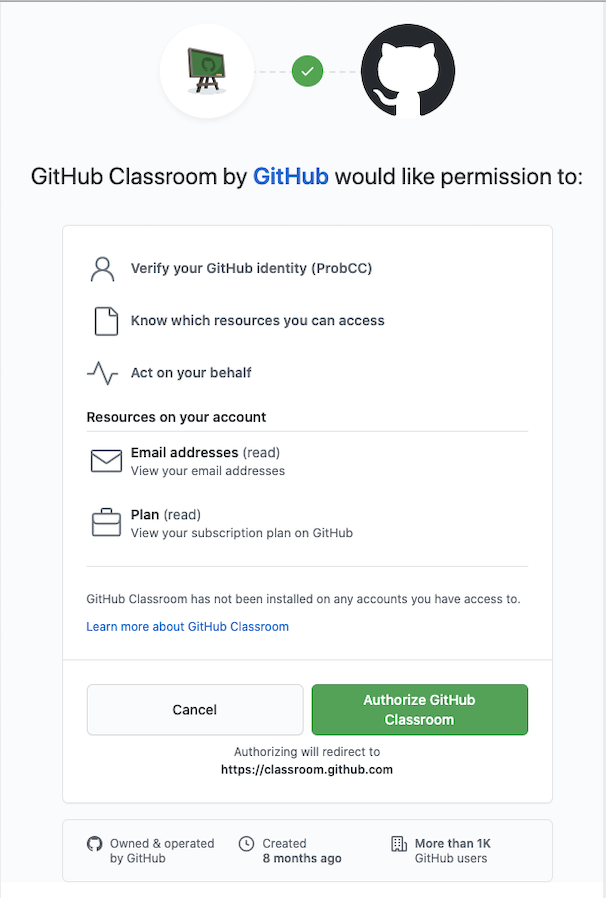
\includegraphics[height=5cm]{figures/github/img01}
  \hspace{1cm}
  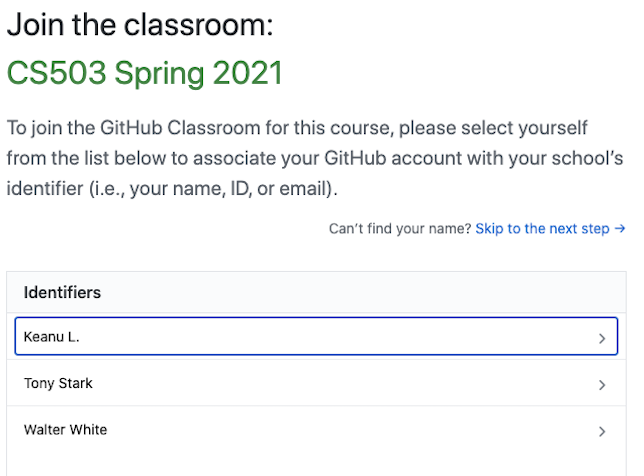
\includegraphics[height=5cm]{figures/github/img02}

\item \textbf{Accept the assignment (Create a team).}
  Use this link \url{https://classroom.github.com/a/VTRXy3E9} to accept the assignment on github classroom.

  The first person in a team accepting the assignment need to create a team. Please use your group name on Brightspace as your team name (e.g. group1). Other team members should find and join the team.

  You should see screens similar to these:

  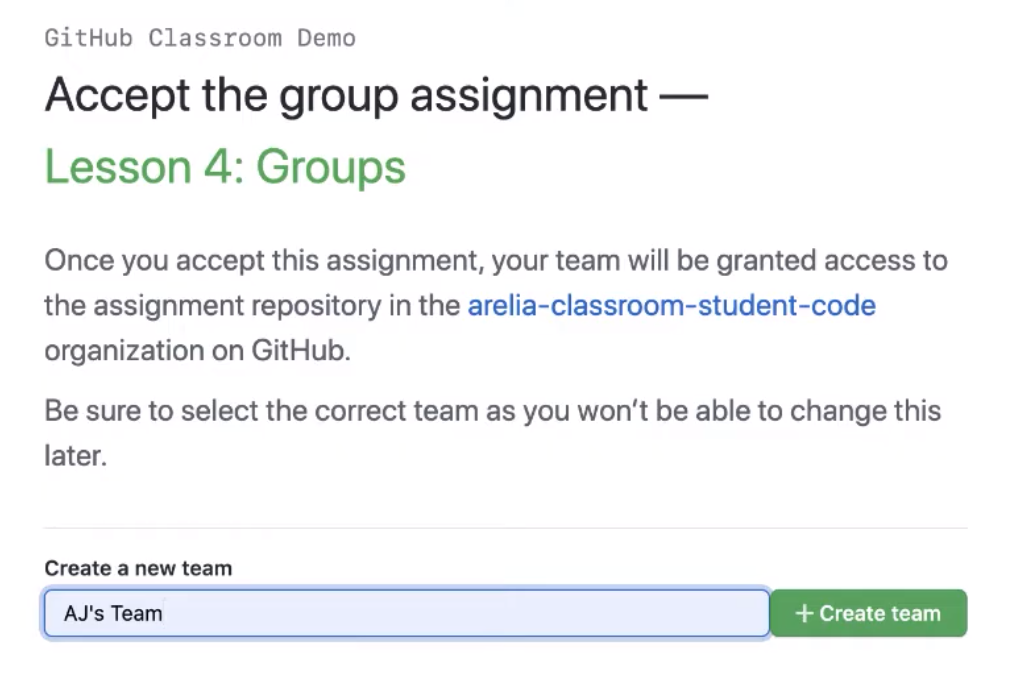
\includegraphics[height=5cm]{figures/github/img05}
  \hspace{1cm}
  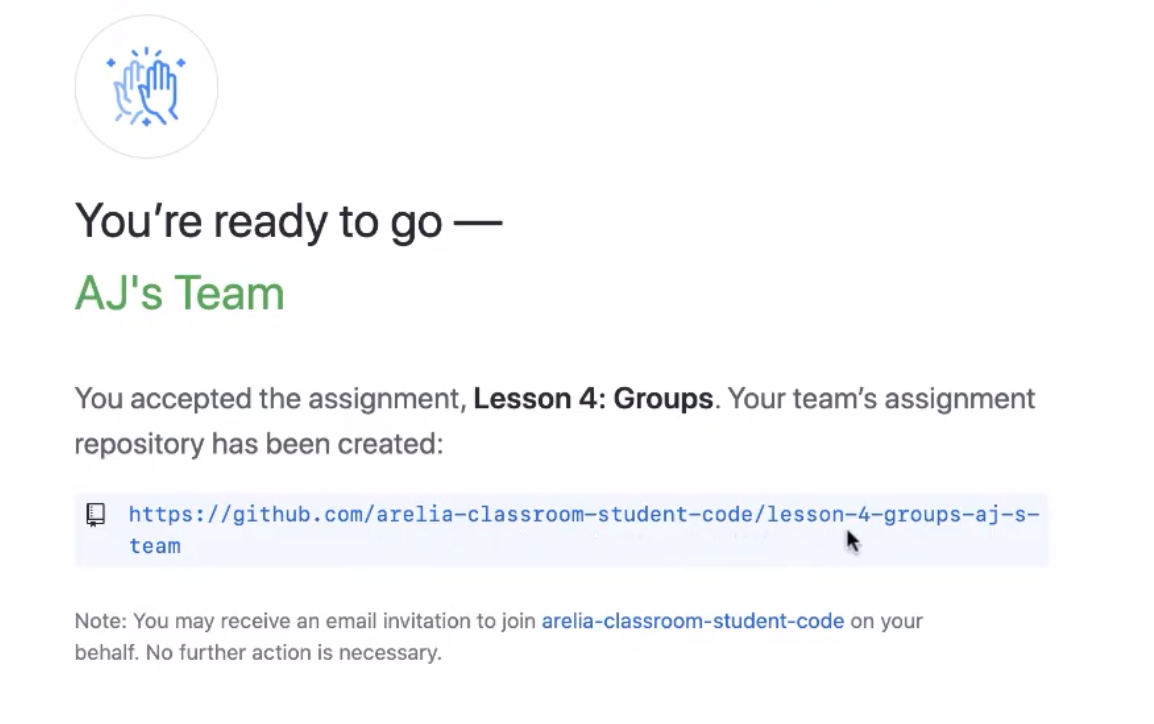
\includegraphics[height=5cm]{figures/github/img06}

\item \textbf{Accept the assignment (Join a team).}

You should see screens similar to these:

  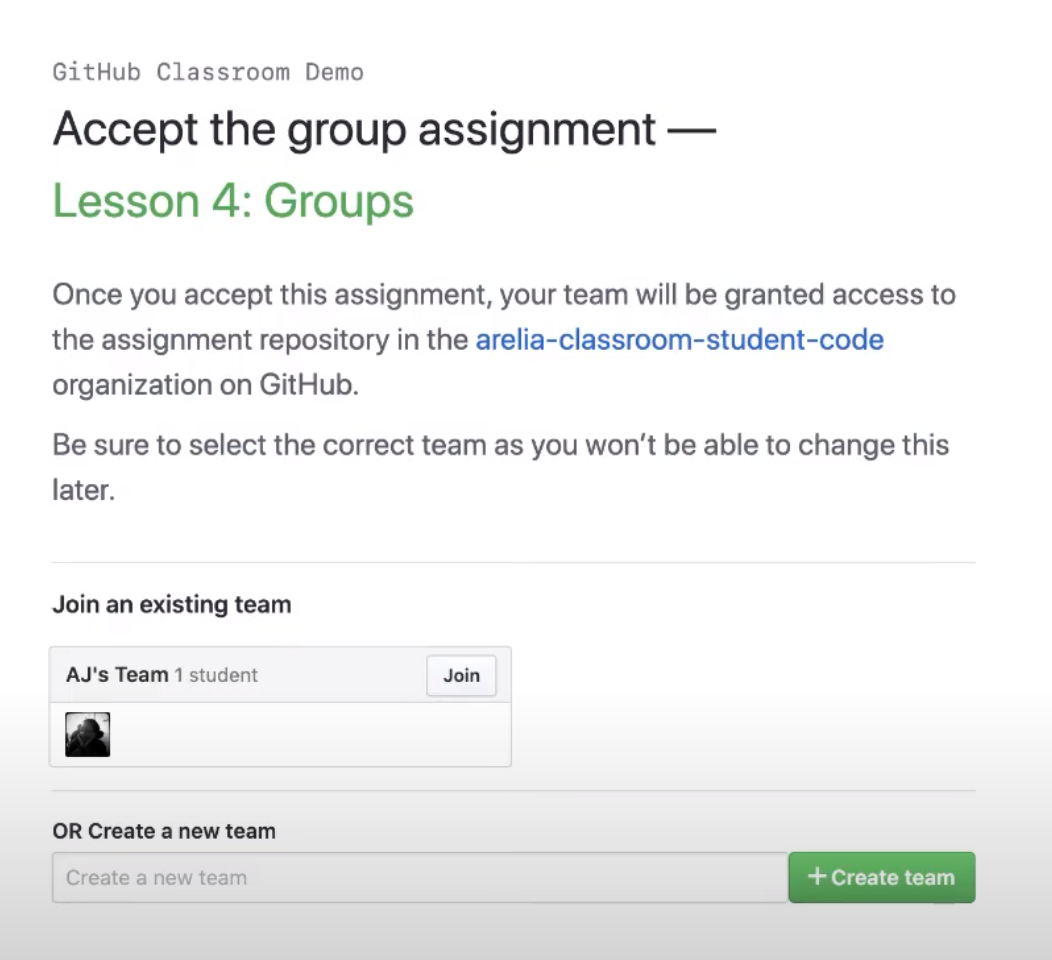
\includegraphics[height=5cm]{figures/github/img07}

Find your team and click join.

\item \textbf{Get you repo URL.}
  As the image shows, your project repository will have the
  format:\\
  \url{https://github.com/cs408-spring-2026/<projectName>-<yourTeamName>/}
\end{enumerate}

\subsection{Development workflow}
\label{development-workflow}

In case you forget the project repository name, you can go to
\url{https://github.com/cs408-spring-2026} to find it. For illustration
purposes, we will \textbf{assume} that your project is under
\emph{https://github.com/cs408-spring-2026/Lab-1---Group-123} and your team's name is
\textit{Lab 1 - Group 123}, so please adjust the links/directories accordingly.

\begin{enumerate}

\item \textbf{Clone the project repository.}

For example, to clone the repository in a new \textit{myclass} folder in your home
directory you should execute the following commands:

\begin{verbatim}
$ mkdir -p ~/myclass/; cd ~/myclass/;
$ git clone git@github.com:cs408-spring-2026/Lab-1---Group-123.git
$ cd Lab-1---Group-123/
\end{verbatim}

This project folder, \emph{Lab-1---Group-123}, would be your
project's \textbf{root directory}.

\item \textbf{Modify the source code as needed.}

% Note that in some cases (e.g., when adding new files) you need to run
% `make clean'`' before `make'  to reload header modifications, otherwise
% your build might be incomplete.

\item \textbf{Commit and push changes to the private Github server repo regularly.}

Note that you are required to regularly commit and push your changes to the private git
in github classrooms.

\begin{verbatim}
$ git commit
$ git push
\end{verbatim}

\end{enumerate}

\section{Useful Libraries and algorithms}
\label{sec:appx:libs}

\subsection{POSIX threads and synchronization operations}
\label{subsec:appx:pthreads}

In Linux, multi-threaded programs generally rely on the \pthread library to
manage threads and execute synchronization operations. The \pthread interface
is defined by the 1995 IEEE POSIX 1003.1c standard.

For this project, you will need to understand the main functions of
\pthread library that are listed in this section. Note that, of all \pthread
operations defined by the standard, you only need to support the \pthread
operations listed in this section. However, you will need to consult
the Linux manual for the detailed semantic of these operations. In
``data.cs.purdue.edu'' and other UNIX systems, you can view the manual with
\texttt{man <function_name>}. You can find a good explanation of these concepts in [8].

You can assume that thread and synchronization objects are initialized with
default attributes and options by the program unless otherwise noted.

\para{Thread management}

\begin{itemize}
\ttit{int pthread_create(pthread_t *thread, const pthread_attr_t *attr,
                         void *(*start_routine) (void *), void *arg)}
\ttit{void pthread_exit(void *retval)}
%\ttit{int pthread_join(pthread_t thread, void **retval)}
\ttit{int pthread_yield(void);}
\end{itemize}


\para{Condition variables}

\begin{itemize}
\ttit{int pthread_cond_wait(pthread_cond_t *cond, pthread_mutex_t *mutex)}
\ttit{int pthread_cond_signal(pthread_cond_t *cond)}
\ttit{int pthread_cond_broadcast(pthread_cond_t *cond)}

%\ttit{int pthread_cond_timedwait(pthread_cond_t *cond, pthread_mutex_t *mutex, const struct timespec *abstime)}

%\ttit{int pthread_cond_timedwait(pthread_cond_t *cond, pthread_mutex_t *mutex, const struct timespec *abstime);}
\end{itemize}



\para{Mutexes}
\begin{itemize}
\ttit{pthread_mutex_lock(pthread_mutex_t *mutex)}
\ttit{pthread_mutex_unlock(pthread_mutex_t *mutex)}
\ttit{int pthread_mutex_trylock(pthread_mutex_t *mutex)}
\end{itemize}


\if 0
\para{Read/write locks}
\begin{itemize}
\ttit{int pthread_rwlock_rdlock(pthread_rwlock_t *lock)}
\ttit{int pthread_rwlock_wrlock(pthread_rwlock_t *lock)}
\ttit{int pthread_rwlock_unlock(pthread_rwlock_t *lock)}
\ttit{int pthread_rwlock_tryrdlock(pthread_rwlock_t *lock)}
\ttit{int pthread_rwlock_trywrlock(pthread_rwlock_t *lock)}
\end{itemize}
\fi

\subsection{Dynamic interception of library calls}
\label{subsec:appx:ldpreload}

\para{LD_PRELOAD instrumentation.}
The Linux dynamic loader, ld-linux, searches and loads shared library files
required by a loaded program at runtime.
\ldp is an optional \textit{environment variable} used by ld-linux.
The loader will load the shared link library specified by
\ldp before any other libraries are loaded, including the C language runtime
(\textit{glibc}). The process of loading libraries with \ldp is
called preloading and is often used to intercept library calls made by a
target program easily.

Preloading means that the functions will be called before the function of the
same name in other library files so that the (original) library functions can be blocked
or replaced. Multiple shared link library files can be provided by separating their paths
with colons or spaces.

To avoid malicious attacks, the loader does not preload libraries using
\ldp when the real user id (ruid) is different from the effective user id
(euid). This mechanism prevents a (non-privileged) user from changing the behavior of a
program when not allowed to do so. In practice, this mechanism is unlikely to affect you
because binaries directly produced by gcc will have the real user id.

Refer to the Linux man page for additional details about the loader using
\textit{man ld-linux}.

\para{A simple LD_PRELOAD example.} The following code illustrates how simple
it is to replace a library call using the \ldp method.

Consider a simple testing library that redefines the \textit{rand()} function:
\begin{verbatim}
  // testlib.c (testing framework)
  int i;
  int rand(){
      return i++;
  }
\end{verbatim}

And consider a simple target program:
\begin{verbatim}
  // target_program.c (target program)
  #include <stdio.h>
  #include <stdlib.h>
  #include <time.h>

  int main(){
    srand(time(NULL));
    int i = 5;
    while(i--){
      printf("%d\n", rand()%100);
    }
    return 0;
  }
\end{verbatim}

The next step is to compile the code above to a shared library and define the
\ldp environment variable to point to the testing library.
Use absolute
paths or ensure that the library can be found through a relative path from the
current working path.

Compiling and running the original target program produces a list of 5 random numbers:
\begin{verbatim}
  $ gcc -o target_program target_program.c
  $ ./target_program
  60
  95
  55
  53
  82
\end{verbatim}

However, if we load the testing library using the \ldp method when running the program,
the results of the same target program become deterministic:
\begin{verbatim}
  $ gcc -shared -fPIC testlib.c -o testlib.so
  $ LD_PRELOAD=testlib.so ./target_program
  0
  1
  2
  3
  4
\end{verbatim}

This simple example shows that with this approach, a testing framework can
control non-deterministic events, e.g., the result of the rand() library call,
and make them deterministic.

Note that using \ldp you are changing program behavior. Depending on how
you change the program, it could lead to data loss or other unexpected results.
Hence, backup your data beforehand and be careful with the library code.

\para{Interposing with LD_PRELOAD.}
When the goal is not to replace a library function but instead to run additional code
and still call the original library function, we need to also invoke
the original library
function from the \textit{testing library}.

Invoking the original library
function involves the following steps:
(a) finding out the address of the
original library function with dlsym(),
(b) saving the value in a function pointer variable,
and (c) invoking the function pointer. This process is shown in the following
example:

\begin{verbatim}
  #define _GNU_SOURCE
  #include <dlfcn.h>
  
  typedef int (*rand_func_t)(void);
  
  int rand(void)
  {
      rand_func_t orig_rand_func;
  
      orig_rand_func = dlsym(RTLD_NEXT, "rand");
  
      return orig_rand_func() % 2;
  }
\end{verbatim}

Running the target program with testlib2 would show that now the non-determinism of the original program has been reduced because of the module 2 operation on the original rand() function.
\begin{verbatim}
  $ gcc -shared -fPIC  testlib2.c -o testlib2.so -ldl
  $ LD_PRELOAD=testlib2.so ./target_program
  1
  1
  1
  1
  0
\end{verbatim}

In practice, dlsym() would have to be used not just when the library needs to call
the original rand() function, within the replaced function, but also every time
the library needs to call the original rand() function for any other reason.
For instance, the library may need to call the original rand() to initialize variables,
such as the starting point of a different ``random'' oracle.

% Removed: 09/09/2025 due to simplfy the questions
%\subsection{PCT Algorithm Work Flow}
%\label{subsec:appx:pct}
%\vspace*{3pt}
%\para{Initialization.}
%At the start of the program execution, your testing library should assign a
%random priority to each program thread, including those not yet
%created. To achieve this, we will assume that there will not be more than 64 threads during the entire program execution. Hence, you should initialize an array \textit{priority} with 64 integers with \textit{priority[i] = i} and then randomly shuffle it with the following code:
%
%\begin{verbatim}
%  void shuffle(int *array, size_t n)
%  {
%      if (n > 1)
%      {
%          size_t i;
%          for (i = 0; i < n - 1; i++)
%          {
%            size_t j = i + rand() / (RAND_MAX / (n - i) + 1);
%            int t = array[j];
%            array[j] = array[i];
%            array[i] = t;
%          }
%      }
%  }
%\end{verbatim}
%
%The \textit{priority} array will maintain the priority of each thread, where
%the array index is the thread sequential number, and the array value is the thread priority.
%Higher values represent higher priority.

% You can run the initialization code in the testing library constructor in the utils.c.


%% removed 09/12/2025 due to remove PCT algo
%\subsection{Thread schedule details}
%
%\vspace*{3pt}
%\para{Controlling thread schedule.}
%After initialization, your testing library needs to know which threads are runnable at every scheduling point.
%And of the runnable threads, it should always run the highest priority thread.
%Threads that are \textbf{blocked} on a mutex or a conditional variable are not runnable; every other existing thread is runnable.
%
%The identification of the next thread to run, blocking of the current thread, and unblocking of the next thread needs to be done for all \pthread calls and also when threads start and when threads terminate.
%The exact method depends on the synchronization method type (mutex vs. conditional variable) as described below.
%
%Of the threads that are runnable, your testing library should pick the highest priority one to run (and only that one should be allowed to run).
%You should implement this using additional synchronization operations that your library performs in a controlled manner.
%The simplest approach is to use an array of semaphores, one for each thread, and selectively call \textit{sem_wait} and \textit{sem_post} on them.
%The following sections provide an overview of how this can be achieved for the two classes of synchronization operations.

%\vspace*{3pt}
%\para{Mutexes.}
%To determine whether threads would block or not on mutexes, the testing library should use \textit{pthread_mutex_trylock}.
%In particular, your library needs to intercept
%the calls to \textit{pthread_mutex_lock}, but
%it must not call the original function immediately because this function can cause the threads to block. Hence, the testing library should do the following inside the \textit{pthread_mutex_lock} test library function:
%
%\begin{enumerate}
%  \item Store the mutex object used by the \textit{pthread_mutex_lock} function in a global array, but do not call the original \pthread function at this point.
%  \item Identify which thread should be allowed to run next.
%  \item Unblock the thread that should run next (e.g., \textit{sem_post}).
%  \item Block the current thread using a per-thread testing semaphore (e.g., \textit{sem_wait}).
%  \item Call the original \textit{pthread_mutex_lock} functions.
%\end{enumerate}
%
%To identify the thread that should run next, your testing library must call
%\textit{pthread_mutex_trylock} on the respective object for all threads with outstanding \textit{pthread_mutex_lock} invocations. This will identify the runnable threads regarding mutexes.
%Then your code should select the non-blocked thread that has the highest priority based on the \textit{priority} array.
%In practice, this process ensures that the original \textit{pthread_mutex_lock} function is only called when the testing tool knows that it will not block.
%
%\vspace*{3pt}
%\para{Conditional variables.}
%For the conditional variable functions (i.e., \textit{pthread_cond_wait}, \textit{pthread_cond_signal}, and \textit{pthread_cond_broadcast}) you will need to model them in the testing library, without calling the original \pthread functions.
%This will be more complex than addressing the mutex operations.
%In particular, it will require implementing a queue of threads for each conditional variable.
%Threads that called \textit{pthread_cond_wait} but have not yet been signaled with \textit{pthread_cond_signal} or \textit{pthread_cond_broadcast} by another thread should be placed in the respective conditional variable waiting list.
%
%For this project, assume FIFO semantic for conditional variables.
%Hence, when a thread calls \textit{pthread_cond_signal} and multiple threads are blocked on the respective conditional variable the first thread that called \textit{pthread_cond_wait} is the one unblocked. \textit{pthread_cond_broadcast} unblocks all threads waiting on the conditional variable.
%\pf{This is also not relevant.}
%
%\vspace*{7pt}
%\para{Additional resources.}
%You can find more information about this algorithm in [6]. However, for this assignment, you do not need to implement priority inversion points. \pf{Not relevant}

\section*{References}

\noindent [1] \url{https://catonmat.net/simple-ld-preload-tutorial}\\
\noindent [2] \url{https://ctf-wiki.github.io/ctf-wiki/reverse/linux/ld_preload/}\\
\noindent [3] \url{https://github.com/libunwind/libunwind}\\
\noindent [4] \url{https://www.nongnu.org/libunwind/}\\
\noindent [5] \url{https://hpc-tutorials.llnl.gov/posix/}\\
\noindent [6] A Randomized Scheduler with Probabilistic Guarantees of Finding Bugs.
\url{https://www.microsoft.com/en-us/research/wp-content/uploads/2016/02/asplos277-pct.pdf} \\
\noindent [7] Program Library HOWTO.
\url{https://tldp.org/HOWTO/Program-Library-HOWTO/miscellaneous.html}\\
\noindent [8] Thread API chapter. \url{http://pages.cs.wisc.edu/~remzi/OSTEP/threads-api.pdf}\\
\noindent [9] \url{https://www.gnu.org/software/libc/manual/html_node/Process-Completion-Status.html}\\
\noindent [10] \url{https://man7.org/linux/man-pages/man7/signal.7.html}



%\newpage
%\bibliographystyle{abbrvnat}
%\bibliography{n-str,p,n}

\end{document}
